\documentclass[sigconf]{acmart}

\usepackage{comment, graphicx, algorithm, algorithmic, listings}


\lstdefinelanguage{P4}{
  showlines=true,
  morecomment=[f]{//},
  keepspaces=true,
  basicstyle=\scriptsize\ttfamily,
  emphstyle=\itshape,
  emph={},
  commentstyle=\color{red},
  keywordstyle=\color{blue},
  morekeywords={typedef, header, extern, struct, parser, state, transition, in, out, inout, select, default, control, action, table, apply, if, switch}
}

\lstdefinelanguage{asm}{
  showlines=true,
  morecomment=[l]{//},
  keepspaces=true,
  basicstyle=\scriptsize\ttfamily,
  emphstyle=\itshape,
  emph={},
  commentstyle=\color{red},
  keywordstyle=\color{blue},
  morekeywords={load, const, invoke, ifeq, pop, add, return, code, data}
}

\lstdefinelanguage{cond}{
	showlines=true,
	morecomment=[l]{//},
	keepspaces=true,
	basicstyle=\scriptsize\ttfamily,
	emphstyle=\itshape,
	emph={},
	commentstyle=\color{red},
	keywordstyle=\color{blue},
	morekeywords={Pre, Post, valid, invalid}
}

\AtBeginDocument{%
	\providecommand\BibTeX{{%
			\normalfont B\kern-0.5em{\scshape i\kern-0.25em b}\kern-0.8em\TeX}}}

%% Rights management information.  This information is sent to you
%% when you complete the rights form.  These commands have SAMPLE
%% values in them; it is your responsibility as an author to replace
%% the commands and values with those provided to you when you
%% complete the rights form.
\setcopyright{acmcopyright}
\copyrightyear{2018}
\acmYear{2018}
\acmDOI{10.1145/1122445.1122456}

%% These commands are for a PROCEEDINGS abstract or paper.
%%\acmConference[Woodstock '18]{Woodstock '18: ACM Symposium on Neural
%%  Gaze Detection}{June 03--05, 2018}{Woodstock, NY}
%%\acmBooktitle{Woodstock '18: ACM Symposium on Neural Gaze Detection,
%%  June 03--05, 2018, Woodstock, NY}
%%\acmPrice{15.00}
%%\acmISBN{978-1-4503-XXXX-X/18/06}

\begin{document}
	
	
	\title{TODO}
	
	
	\author{}
	\email{}
	\orcid{}
	\author{}
	\authornotemark[]
	\email{}
	\affiliation{%
		\institution{}
		\streetaddress{}
		\city{}
		\state{}
		\country{}
		\postcode{}
	}
	
	
	\begin{abstract}
		TODO
	\end{abstract}
	
	%%
	%% The code below is generated by the tool at http://dl.acm.org/ccs.cfm.
	%% Please copy and paste the code instead of the example below.
	%% TODO

	
	\keywords{TODO}
	
	
	\maketitle
	
	\section{Introduction}
	  Optimization, verification and refactoring are important tasks of a software development process. All of them can be effectively supported by static functional and non-functional (e.g. execution time estimation) analysis. These analysis can be especially interesting in the case of languages having uncommon language constructs or language structures e.g. in the case of some domain specific languages. 
	
	
	% P4 (max 1-1.5 hasáb) - példa (később használandó a többihez) - Máté
	P4~\cite{p4paper} is a high level, domain-specific programming language. It is developed mainly for
describing the data plane layer of packet processing algorithms of different network
devices (e.g. switches, routers) in a protocol and target independent way. Figure~\ref{code:P4} illustrates a P4 program. The program first defines the applied header structure, than the parser part describes how the fields of the defined headers will be set from the input bit stream (input packet). Controller part can modify values of fields of headers and metadata by applying lookup tables. The data plane program describes the structure of the tables, the key fields based on that lookups will be executed and the possible results of the lookups, namely the applicable actions. However concrete data of the tables (which actions will be executed with which parameters for which key values) are defined by the control plane program, therefore it will not appear in P4. Finally the deparse part defines how the output bit stream (output packet) will be created from the headers.   
	
	The paper describes an analysis framework for P4. The framework makes possible development of different P4 related analysis methods in a generic and modular way. It uses an internal graph representation where the results of the methods are also represented as part of the graph (mainly by adding new edges to the graph). In this way the methods can use each other's results as well.  

\begin{figure*}
\begin{tabular}{|p{3.3cm}|p{5.9cm}|p{7.7cm}|}
\hline
\begin{lstlisting}[language=P4]
// Definitions
typedef bit<9>  egSpec_t;
typedef bit<48> macAddr_t;
typedef bit<32> ip4Addr_t;

// Headers
header ethernet_t {
  macAddr_t dstAddr;
  macAddr_t srcAddr;
  bit<16>   etherType; }
    
header ipv4_t {
  bit<8>    ttl;
  ip4Addr_t srcAddr;
  ip4Addr_t dstAddr;... }
    
struct headers {
  ethernet_t   ethernet;
  ipv4_t       ipv4; }

\end{lstlisting}
&
\begin{lstlisting}[language=P4]
// Parser
parser MyParser(...) {
  state start { transition parse_ethernet; }
  state parse_ethernet {
    packet.extract(hdr.ethernet);
    transition select(hdr.ethernet.etherType) {
      TYPE_IPV4: parse_ipv4;
      default: accept; } }
  state parse_ipv4 {
    packet.extract(hdr.ipv4);
    transition accept; } }
    
// Control    
control MyIngress(in headers hdr, ...) {
  apply {
    if (hdr.ipv4.isValid()) {
           ipv4_lpm.apply(); }
  }         
  action drop() {
    mark_to_drop(standard_metadata);
  }    
\end{lstlisting}
&
\begin{lstlisting}[language=P4]
  action ipv4_forward(macAddr_t dstAddr, egSpec_t port) {
    standard_metadata.egress_spec = port;
    hdr.ethernet.srcAddr = hdr.ethernet.dstAddr;
    hdr.ethernet.dstAddr = dstAddr;
    hdr.ipv4.ttl = hdr.ipv4.ttl - 1;
  }    
  table ipv4_lpm {
    key = {  hdr.ipv4.dstAddr: lpm;  }
    actions = {
      ipv4_forward;
      drop;
      NoAction;}
    ... }   
}

//Deparser
control MyDeparser(packet_out packet, in headers hdr) {
  apply {
    packet.emit(hdr.ethernet);
    packet.emit(hdr.ipv4);}
}
\end{lstlisting}\\
\hline
\end{tabular}
\caption{P4 example}
  \label{code:P4}
\end{figure*}


	
	
	\section{Related Work}
	% kb 1.5 hasáb
	% felhasznált eszközök  - 
	% egyéb toolok - Vera,  - Gabi
	% Akár gremlin/gráf alapú dolgok, ami nem p4 (akár refactorerl) - mindenki
	
	\subsection{Used tools}

  In the tool architecture described in Section~\ref{sec:rep}, we use a Gremlin graph database as storage backend (knowledge graph). Gremlin is a compositional query language and API that is implemented by many large-scale graph databases. This makes it possible to change graph implementations with almost no modification to the <NAME> code base at all. In earlier work~\cite{icai20}, we also profiled a few graph backends for control flow traverals. 
  Another consequence is that analysers have to be implemented as graph query workflows. By coarsely granularizing queries, most of the work can be delegated to the database, and with this, the choice of the workflow language (e.g. Java) can become negligible. In earlier work~\cite{macs20}, we experimented with implementing a whole control flow analysis as a single graph query: while having advantages, it can also hinder code maintainability as queries are often more difficult to read and modify. 


	\subsection{Similar tools}	
	
	%verification
	
	Considering related work there are many research applying specific analysis technics for P4. Most of them concentrate on error checking of P4 programs. For example Assert-P4 \cite{assertp4} and Vera \cite{vera} ask annotated P4 source from the developer and with symbolic execution they check if the predefined properties are correct during the program, although Vera can also detect common errors without annotations. P4V \cite{p4v} creates a formula, which describes the proper behavior of the program and checks the satisfiability of it with SMT solver. These tools are created for an earlier version of P4, namely P4$_\text{14}$. There are also verification tools, which can manage the newer version (P4$_\text{16}$) too. BF4 \cite{bf4} is created as a p4c backend, which can not only detect error possibilities, but it is able to repair them by adding new keys to the table and modify the table contents. An other tool p4-data-flow \cite{p4dataflow} uses data flow analysis to detect potential bugs in P4 switch codes.
	These tools use static analysis, but there are other approaches too. P4RL \cite{p4rl} works with the programs at runtime and its verification is based on fuzzing and reinforcement learning techniques.
	Some other tools uses analysis methods for different purposes. For example p4pktgen \cite{p4pktgen} uses symbolic execution for automatically generating test cases. Flightplan \cite{flightplan} can splits a P4 program into a set of cooperating P4 programs and maps them to run as a distributed system formed of several, possibly heterogeneous, dataplanes. During this process they use several analysis technics, for example to gather variables whose values must be transfer between dataplanes. 

	 
	
	Our solution is a general tool which contains several analyzes.	
	
	The approach of the graph-based static analysis of programs is well-known. It is used wide ranged for example with Java \cite{9064792}, 
	
	
	
  %graph-based
  % - refactorerl
  
  %gremlin-based
  % - An Efficient and Scalable Platform for Java Source Code Analysis Using Overlaid Graph Representations: https://core.ac.uk/download/pdf/323304005.pdf
  % - Graph-based Vulnerability Detection via Extracting Features from Sliced Code: https://qrs20.techconf.org/QRSC2020_FULL/pdfs/QRS-C2020-4QOuHkY3M10ZUl1MoEzYvg/891500a038/891500a038.pdf
  % - Application of Graph Databases for Static Code Analysis of Web-Applications: http://ceur-ws.org/Vol-2590/short30.pdf
  % - Efficient and Flexible Discovery of PHP Application Vulnerabilities: https://fabs.codeminers.org/papers/2017b-eurosp.pdf
  % -  Modeling and Discovering Vulnerabilities with Code Property Graphs: https://fabs.codeminers.org/papers/2014-ieeesp.pdf , slides: http://mlsec.org/joern/docs/2014-inbot.pdf
  % - Reverse Engineering State and Strategy Design Patterns using Static Code Analysis: https://thesai.org/Downloads/Volume9No1/Paper_78-Reverse_Engineering_State_and_Strategy_Design_Patterns.pdf


	\section{Motivation}
	% max 1 hasáb - lehet intorba megy - Máté
	% p4-re vannak elemzések kéne fejlesztés segítő eszköz
	% ehhez egységes keretrendszer - vannak már ilyesmik related workben
	

  %% p4c is a factory. this tool is a laboratory. 



	\section{Analysis framework}


Traditional compilers are designed around passes: the frontend passes parse source code into an intermediate representation (IR), midend passes transforms and adds new information to the IR, and the backend passes create target-specific object code from the IR~\cite{trad-compilers}.  
Modular compilers like P4C improve this design by structuring the passes into a library: backends assemble their own frontends and midends from a catalogue of passes provided by the compiler. Moreover, P4C allows getting information from older states of the IR, as each transformation pass returns an immutable IR instance.
Even here, the three-fold separation of frontend-midend-backend have to remain: in order satisfy midend-dependencies, and subsequently, backend-dependencies, the backend must sequentially execute the frontend, the midend, and finally its own passes. 

One goal of the experiment we present here is to relax the three-fold structure and allow passes to reuse (depend on) each other's functionally arbitrarily, and without burdening the compiler programmer with manually finding the right sequence in which to execute these dependencies.

\subsection{Representation - Architecture}\label{sec:rep} % 4 hasáb - Dániel
	% belső gráf, a koncepció
	% elemzések
	% app megvalósítás


  \begin{figure}
    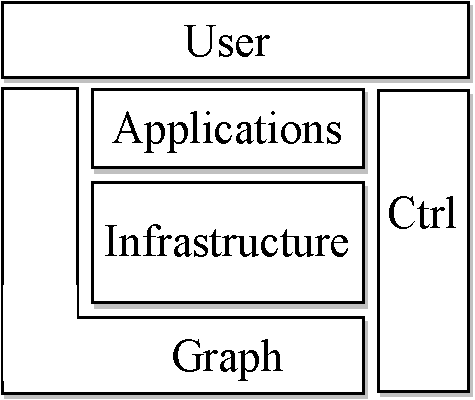
\includegraphics[width=0.18\textwidth]{figures/arch-top.pdf}
    \caption{TODO}\label{fig:arch-top}
  \end{figure}

Besides proposing a more relaxed structure of analysis passes, we had three additional goals in sight: support for different applications through uniform APIs, ease of extensibility, and data-driven programming.

By \textit{supporting different applications} (or backends, in compiler parlance), we mean providing a comfortable way to to implement different end-users services, by reusing the same static code analysis operations.
See Section~\ref{fig:apps} for a few examples of applications built on top of the <NAME>.
In systems with uniform APIs, programmers have to learn only one paradigm to maintain, extend or otherwise alter the system (e.g. in case of P4C, visitors and passes are the main concepts of such a uniform API). 

Figure~\ref{fig:arch-top} depicts how the architecture of <NAME> realizes uniform APIs by relying on a graph database. 
Superficially, applications provide services to the user, by using the services provided by the infrastructure (see Section~\ref{fig:infra}). In reality, both the infrastructure and applications operate on a large shared graph that collects all our knowledge about the program code. The graph is also exposed to the user to enable custom features (e.g. to attach external loggers, visualisers, and validators). The information in the knowledge graph is accessed using graph queries written in Gremlin (see Section \ref{sec:gremlin}). The implication is that users, application developers, and infrastructure developers are using one, uniform data structure, and are accessing it using the same mechanism. The seamless collaboration of all these components is managed by the controller component.

  \begin{figure}
    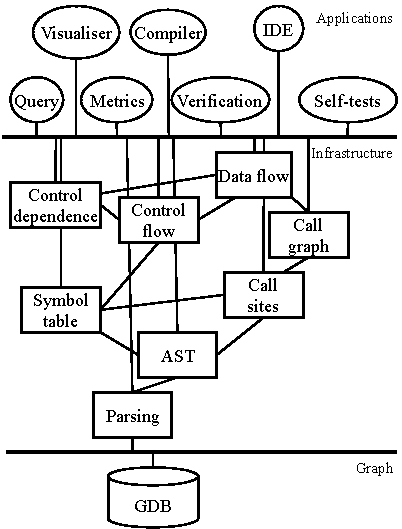
\includegraphics[width=0.3\textwidth]{figures/arch-deps.pdf}
    \caption{TODO}\label{fig:arch-deps}
  \end{figure}

Our second design goal, \textit{ease of extensibility} is illustrated by Figure~\ref{fig:arch-deps}, that elaborates the application and infrastructure layers. 
This arrangement was inspired by declarative build systems and the blackboard pattern used in distributed MI.

The infrastructure consists of a set of interdependent analyser components (or passes, in compiler parlance): higher-level analysers can only be executed when lower-level analysers already inserted the necessary knowledge into the graph. To achieve this, analyser components register their needs and provided services to the controller component, and the controller figures out the topological order in which to initiate the analysers. 
Applications provide a user interface (e.g. command line interface) through which their services can be accessed, and similarly to analysers, applications also depend on a subset of the analysers in the infrastructure. But unlike analysers, application are expected to only read (never modify) the graph, and consequently, applications have no dependents. 
In this arrangement, the controller guarantees that when the user executes a work-intensive application, only the minimally necessary components will be performed.
Moreover, when developers introduce new features, this arrangement enables them to think declaratively: instead of thinking about where to insert their feature inside a sequence of operations, they only have to think about their dependencies, i.e. what kind of analysers could help them.

With this, we arrive to our third design goal, \textit{data-driven programming}. Thanks to the uniform graph API and the controller-managed dependency resolution, programmers are forced to think in terms of data instead of code: they have to look at what code knowledge is in the graph already, figure out what data they want to insert, and possibly find existing analysers that makes writing queries  easier for them. 
The information in the graph is regulated by a well-defined graph schema, and the graph topology is regulated by the well-defined requirements and services of the analysers. Moreover, since the graph instance is detached from the code analysis framework, the programmers can access it by external tools for visualising, monitoring and validating purposes.
Like this, programmers can almost completely avoid understanding the existing code base, and only have to look at and interact with the data in the graph.  
	
	\subsection{Experts} % 1 hasáb - Dániel
	% kisebb gráf ábra
  As we see earlier in Figure~\ref{fig:arch-deps}, the heavy-lifting in <NAME> is done by various code analyser components, each adding new information about the P4 code to the knowledge graph using what is already there. We now introduce a few analyser modules using an example: Figure~\ref{fig:output} depicts a small subset of the knowledge graph taken after we executed control flow analysis, call analysis, and call sites analysis on the P4 code in Figure~\ref{code:P4} (specifically the \texttt{MyIngress} control). 
  First, the controller finds the topological order of their dependencies, and then starts executing them in order. In this case, the first dependency executed is the parser, parsing the P4 code and filling the knowledge graph with the syntax tree nodes and edges. 

  Each analyser components adds new edges as an overlay graph. These overlays (domains) are separated by the \texttt{dom} edge-attributes: for example \texttt{CFG} is the domain introduced by the control flow analysis, and \texttt{CALL} is the domain of the call analysis, \texttt{SITES} is that of call site analysis. The \texttt{role} edge-attribute describes edge semantics inside their domain. For example, \texttt{calls} in \texttt{CALL} links a procedure to those procedures that it calls (e.g. \texttt{MyIngress} control calling \texttt{ipv4\_lpm} table lookup). On the other hand, \texttt{calls} in \texttt{SITES} links call statements (the \textit{direct application} of table \texttt{ipv4\_lpm}) to the called procedure (table \texttt{ipv4\_lpm}). 
  
  At the same time, the \texttt{CFG} domain contains \texttt{flow}, \texttt{entry}, and \texttt{return} edges (among others) to denote the flow of control between various nodes of the syntax tree, and to identify entry and exit nodes. For example, by following these edges, you can see how control flows from the \texttt{MyIngress} entry point through the conditional, terminating on the call of \texttt{ipv4\_lpm}. (For more information on how we implemented control flow analysis using Gremlin, see~\cite{macs20}.) The figure also partially includes domains of other analysers, such as \texttt{SYMBOL}. This analysers creates the graph-equivalent of a symbol table by identifying which declaration declares which name, and links usages of this name in the scope of the declaration to the declaration.

  \begin{figure}
    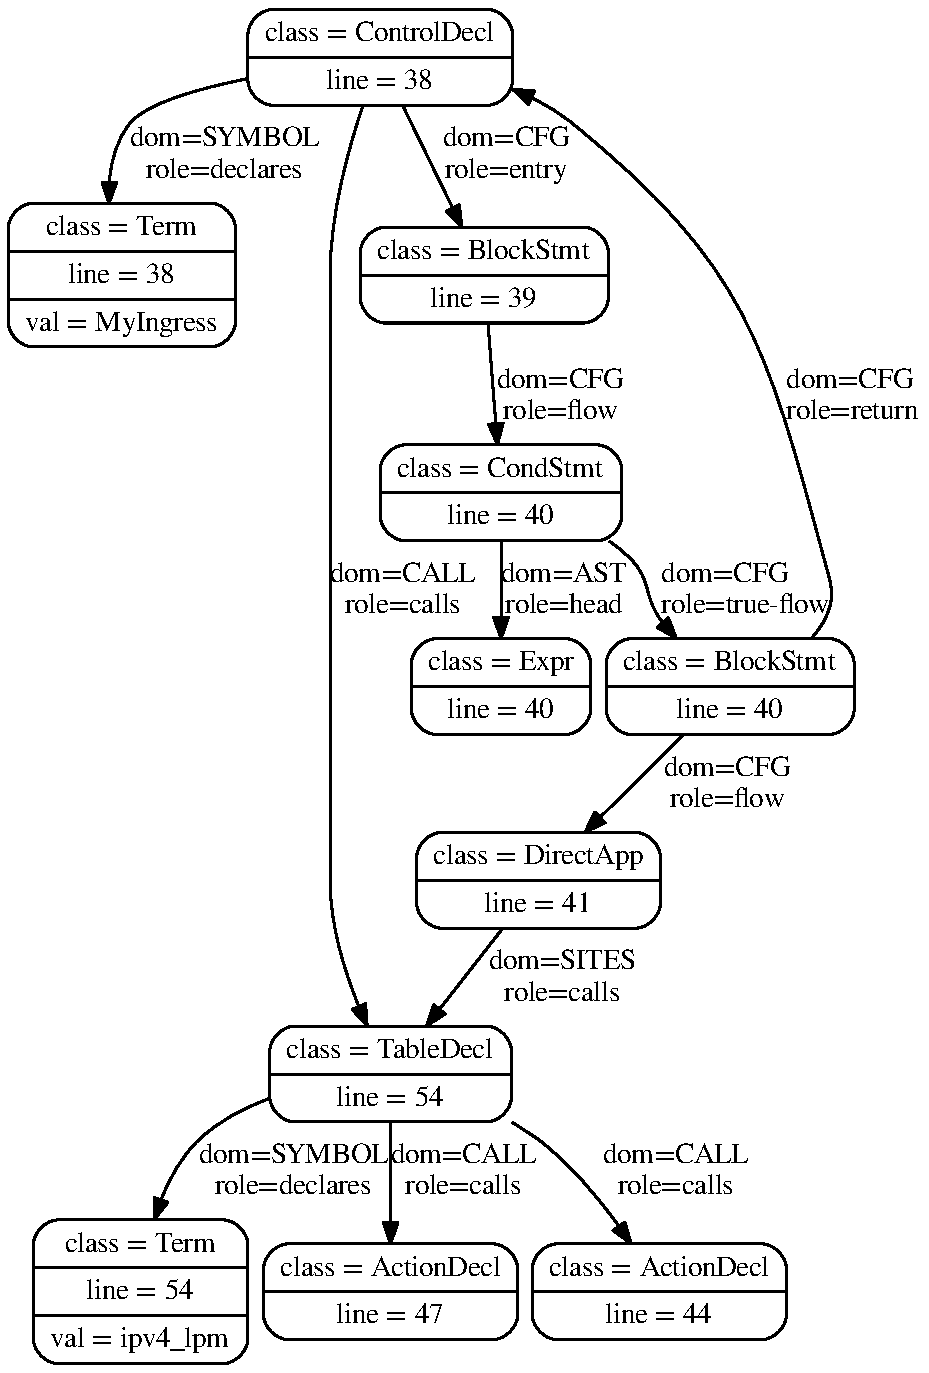
\includegraphics[width=0.45\textwidth]{figures/output.pdf}
    \caption{TODO}\label{fig:output}
  \end{figure}

	\subsection{Testing} % 1 hasáb - Gabi
	There are two main goals with the testing: to test if the analyzes work well; and because it is a quite new tool, it will go through a lot of changes, therefore the possible spoils of the analyses during changes need to be detected. This version of the tool contains unit tests and integration tests to check the functional correctness. 
	
	With the unit tests, our main goal is to check if the analyzes work well. Unit tests need to be fast, therefore they work with the smallest part of the analyses ie. their functions. One function usually define one query of the graph, which insert new edges into it, therefore in these cases, the tests check if the right edges are added to the graph. Using actual P4 source, to test these functions, would be too costly, therefore we define the most simple graphs --, which contains only those edges and vertices, which are necessary for the query -- to check the function.
	
	While unit tests need to be fast, integration tests can be slower, so we can use P4 files as the inputs to test the analyzes. When one analysis needs to be tested, it uses the P4 file, and executes every analysis, that it is based on and the tests will check the result of this running. The tests are predefined, therefore we use a file to store the information of the tested sources and analysis -- which file tests which analyzes with which test classes.
	
	There are two approaches to run these tests. One of them executes all of the defined tests -- i.e. it goes through all of the P4 sources and executes the necessary analyzes and tests the their results -- which is useful to test the whole program and identify regression errors. The other focuses only one analysis and it is useful, when someone actually develop that analysis. This approach run only those tests which are relevant for the analysis.
	
	The architecture gives opportunity to insert the test as an application, which depends on all of the tested analyzes, but these are built into the maven. (TODO - ide még jöhetne talán részletessebben)
	
	
	% külön modul
	% elvi részei jelenlenek meg
	% ilyen olyan teszt, messziről melyik hogy
	% külön modul
	% elvi részei jelenlenek meg
	% ilyen olyan teszt, messziről melyik hogy
	
  \section{Evaluation} % ~ case studies?
	
	% scalability measurements  talán 1 hasáb
	% esetleg 1-2 plre hogy futott le - sor alapján? mini mérés
	
	% indítási információk - mindegyiknél /visualisation-nél
	% egyedi elemzések mérése
	\subsection{Visualisation} % 0.5 hasáb
  
  Since its function is the easiest to understand, the first application we introduce is graph visualisation. This application expects a list of analyser component names, executes them, and then, prints a subgraph of the knowledge graph containing only the domains of the analysers in the list. For example, to print the full version of the graph in Figure~\ref{fig:output}, we should run the following command:

  \begin{lstlisting}[language=bash, basicstyle=\scriptsize]
  $ <NAME> draw -A ControlFlow SymbolTable CallGraph CallSites AST
\end{lstlisting}

  The subcommand \texttt{draw} tells <NAME> to run the visualiser, while \texttt{-A} is a flag (defined by the visualiser UI) expects the analyser names that will be passed to the visualiser application. 

  A possibly interesting implementation detail here is that the visualiser technically depends on \textit{all} the analysers defined in <NAME>, since it must be able to visualise anything the user may pass. Yet, we still managed to avoid executing those that are not requested by the user (and not dependencies of the requested ones): we implemented dependency resolution in the controller using Java dependency injection (DI), and DI offers lazy initialization of the dependencies. This way we can filter the analysers and only initialize those that were requested by the user.

  \subsection{Verification} % 1 hasáb - Gabi
  Verification is a possible extension of the tool, which is added to it as an application. The main focus is to detect errors and suspicious cases, which can be caused by the usage of invalid header or uninitialized fields. The goal of this detection is to report these usages for the developer to avoid undefined behaviour in the programs. 
  
  The approach of the checking is defined in our previous paper \cite{ownCheck}, but shortly, it calculates the pre-and post-condition of the different blocks -- i.e the control apply functions, the tables and actions --, the parser and the deparser of the program and based on their results it can detect improper usage of the fields and headers. Three types of cases can be detected: when there are some error cases in a block; when there is any inconsistency between the blocks; and when the need of the parser-deparser is inconsistent with the need of the control function.
  
  In Figure \ref{code:cond}, there is an example condition for the MyIngress. We can see 4 pairs of conditions, because it has 4 possible execution paths - there are three when the condition of the branch is true, and the table executes one of the possible actions i.e. $\mathit{ipv4\_forward}$, $\mathit{drop}$ or $\mathit{NoAction}$, and one when the condition of the branch is false.
  
  \begin{figure}
  	\begin{lstlisting}[language=cond]
  	MyIngress:
  	[
  	// true condition and ipv4_forward
  	  (Pre: 
  	     valid:   [ipv4, ipv4.dstAddr, ipv4.ttl,
  	               ethernet, ethernet.dstAddr],
  	     invalid: [drop],
  	   Post: 
  	     valid:   [ipv4, ipv4.dstAddr, ipv4.ttl,
  	               ethernet, ethernet.dstAddr],
  	     invalid: [drop]),
  	// true condition and drop
  	  (Pre: 
  	     valid:   [ipv4, ipv4.dstAddr],
  	     invalid: [drop],
  	   Post: 
  	     valid:   [drop, ipv4, ipv4.dstAddr],
  	     invalid: []),
  	// true condition and NoAction
  	  (Pre: 
  	     valid:   [ipv4, ipv4.dstAddr],
  	     invalid: [ipv4, ipv4.dstAddr, drop],
  	   Post: 
  	     valid:   [ipv4, ipv4.dstAddr],
  	     invalid: [ipv4, ipv4.dstAddr, drop]),
   	// false condition
   	  (Pre: 
   	     valid:   [ipv4, ipv4.dstAddr],
   	     invalid: [ipv4, ipv4.dstAddr, drop],
   	   Post: 
   	     valid:   [ipv4, ipv4.dstAddr],
   	     invalid: [ipv4, ipv4.dstAddr, drop]), 
   	]
  	\end{lstlisting}
  	\caption{Conditions of \texttt{MyIngress}}
  	\label{code:cond}
  \end{figure}
  
   This calculation is built into the tool as an application. It uses two experts: the call graph and control-flow graph. While traversing through the call graph it can reach calls of tables and actions. When it reaches a call, it starts to traverse through the proper subgraph of the control-flow graph and calculates the conditions of the actual block. Every condition is stored in the graph as a property of the called vertex of the call graph. 
   The implementation gets and saves every information about the program with Gremlin queries.
  
  \subsection{Compiler} % 1 hasáb - Dániel
  In related research~\cite{cscs18,ocs20}, we work on a static cost analysis tool for P4: the tool expects as input a P4 program source code together with execution environment parameters, and outputs various metrics (e.g. execution time, energy efficiency) without actually running the P4 program.

  In the current paper, we will not go into details on how the cost analysis tool calculates these metrics, but the principle is that we decompose the P4 program into primitive instructions whose expected cost is constant and already known. Implementations of P4 externals such as extern calls and lookup tables (e.g. \texttt{packet.extract} and \texttt{ipv4\_lpm} and in Figure~\ref{code:P4}) can also be passed to the tool in the form of these primitive instructions with known costs. 

  From this, it follows that part of the static cost analysis problem reduces to a compilation-and-linking problem. As an experiment, we implemented a compiler to solve this problem as an application in <NAME>. The main reason we chose <NAME>, instead of the much more mature P4C compiler framework was that at first we did not know what kind of representation or code we will need to output: the control and extensibility provided by <NAME> and Gremlin queries gave us tools to experiment and create quick, recyclable prototypes to help us arrive at a final vision. While P4C's safety mechanisms (e.g. C++ static type system) support developing stable software, in case of prototyping and experimentation these same mechanisms are unused, or possibly even slowing down development.

  Our current target representation for cost analysis is a sequential stack machine with an instruction set similar to JVM bytecode. Figure~\ref{code:stack} depicts the compiler output of \texttt{MyIngress} in Figure~\ref{code:P4}. In the figure all values (bits and sizes) are represented as integers (a requirement by our cost analysis approach). Both \texttt{isValid} and \texttt{ipv4\_lpm} have external implementation that had to be linked with the calls. While most P4 targets will not support stack machines, we chose this representation as it is relatively easy to generate, and relatively straightforward to implement. We also believe that as long as we do not count the cost of maintaining the stack, we can still make good cost estimations.
  
  The compiler is built on top of the control flow analyser in <NAME>: we traverse the CFG, and process each node by traversing the syntax tree under the node. We also use the call graph to find which label to jump to when a function is called. Thus, much of the compiler state can be delegated to the persistent knowledge graph, and only very specific data (e.g. instruction labels) and linking requires program state outside the graph.  

  \begin{figure}
  \begin{lstlisting}[language=asm]
data:
  ...
  headers = 149 
  headers.ethernet = 149   // size 114
  ...
  headers.ipv4 = 263 
  headers.ipv4.valid = 263 
  headers.ipv4.size = 264 
  headers.ipv4.srcAddr = 265 
  headers.ipv4.dstAddr = 297
  ...
code:
  ...
  // call isValid(hdr.ipv4) on line 144
  214:  load 0	      // 0: local address of hdr
  215:  const 114     // 114: size of hdr.ethernet
  216:  add           // address of hdr.ipv4
  217:  invoke 144 1		 
  // test isValid return value
  218:  ifeq 224		 
  // call ipv4_lpm(hdr) on line 38
  219:  load 0        // 0: local address of hdr
  222:  invoke 38 1		 
  223:  pop
  // terminate with status OK
  224:  const 0		 
  225:  return 
\end{lstlisting}
\caption{Stack machine code of \texttt{MyIngress}}
  \label{code:stack}
\end{figure}
  
	\section{Conclusion and Future Work} % 1 hasáb - Máté
	
	  The goal of this paper is to introduce our analysis framework for P4 programs, which is based on a huge graph representation of the program. Analysis can be easily inserted into the tool, as an expert, which calculates the proper side information from the main syntax tree, and also stores this new information in it. 
	
	So far, we have three main applications, which use some subgraph -- experts --, but we plan to increase these numbers and extend them. Two near future plans are the dependency graph and the def-use graph from which we could give some more useful information for the developers about their P4 source. The dependency graph will contain the data and control dependencies between the statements, the def-use graph will show which fields are defined and used in which statements. Based on these analyzes we will be able to see more connection between the statements.		
	
	% talán még cost-analysis? slicing? refactor? error correction?	
	
	Our major purpose to create a tool, which can facilitate and support the work of  P4 developers.
	


\bibliographystyle{ACM-Reference-Format}
\bibliography{tool}

\end{document}
\endinput

